\newcommand{\nDog}{\mathit{dog}\xspace}
\newcommand{\nCat}{\mathit{cat}\xspace}
\newcommand{\aSmall}{\mathit{small}\xspace}
\newcommand{\aSniffing}{\mathit{sniffs}\xspace}
\newcommand{\nBreed}{\mathit{beagle}\xspace}


\section{Measuring Expressive Power}\label{sec:technical}

Relational structures are very suitable for representing \emph{situations} or
\emph{scenes}.  A relational structure (also called ``relational model'') is a non-empty
set of objects --the \emph{domain}-- together with a collection of relations, each with a fixed arity.

Formally, assume a fixed and finite (but otherwise arbitrary)
vocabulary of $n$-ary relation symbols.\footnote{
  Constants and function symbols can be represented as relations of
  adequate arity.}
A relational model $\+M$ is a tuple
$\tup{\Delta,\interp{\cdot}}$ where $\Delta$ is a nonempty set, and
$\interp{\cdot}$ is a suitable interpretation function, that is,
$\interp{r} \subseteq \Delta^n$ for every $n$-ary relation symbol
$r$ in the vocabulary. We say that $\+M$ is \emph{finite} whenever
$\Delta$ is finite.  The \emph{size} of a model $\+M$ is the sum
$\#\Delta + \#\interp{\cdot}$, where $\#\Delta$ is the cardinality
of $\Delta$ and $\#\interp{\cdot}$ is the sum of the sizes of all
relations in $\interp{\cdot}$.

Figure~\ref{fig:cat-dog-1} below shows how we can represent a scene
as a relational model. Intuitively, $a$, $b$ and $d$ are dogs, while
$c$ and $e$ are cats;  $d$ is a small beagle;
 $b$ and $c$ are also small.
 We read $\aSniffing(d,e)$ as ``{\em $d$ is sniffing $e$}''.

 \begin{figure}
 \begin{center}
 \begin{tabular}{rcl}
$\Delta$               & = & $\cset{a,b,c,d,e}$\\
$\interp{\nDog}$      & = & $\cset{a,b,d}$\\
$\interp{\nCat}$      & = & $\cset{c,e}$\\
$\interp{\nBreed}$    & = & $\cset{d}$\\
$\interp{\aSmall}$    & = & $\cset{b,c,d}$\\
$\interp{\aSniffing}$ & = & $\cset{(a,a),(b,a),(c,b),(d,e),(e,d)}$
 \end{tabular}
\begin{picture}(120,50)
\put(0,-50){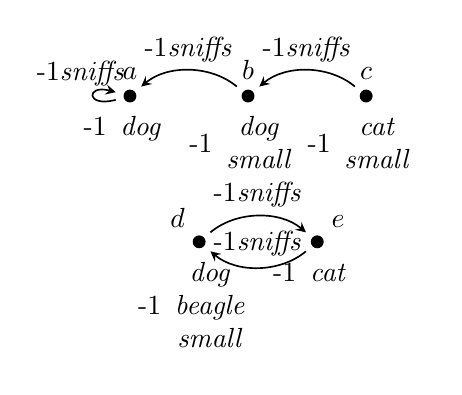
\begin{tikzpicture}
  [
    n/.style={circle,fill,draw,inner sep=1.5pt,node distance=1.5cm},
    aSniffing/.style={->, >=stealth, semithick, shorten <= 3pt, shorten >= 3pt},
  ]
 \node[n,label=above:$a$,label=below:{\relsize{-1}$\begin{array}{c}\nDog\end{array}$}] (a) {};

 \node[n,label=above:$b$,label=below:{\relsize{-1}$\begin{array}{c}\nDog\\ \aSmall \end{array}$}, right of=a] (b) {};

 \node[n,label=above:$c$,label=below:{\relsize{-1}$\begin{array}{c}\nCat\\ \aSmall\end{array}$}, right of=b] (c) {};

 \node[n,label=above left:$d$,label=below:{\relsize{-1}$\begin{array}{c}\nDog\\ \nBreed\\  \aSmall \end{array}$}, below of=a,xshift=25pt,yshift=-10pt] (d) {};

 \node[n,label=above right:$e$,,label=below:{\relsize{-1}$\begin{array}{c}\nCat\end{array}$},right of=d] (e) {};

 \draw [aSniffing,loop left] (a) to node[above,xshift=-5pt]{\relsize{-1}$\aSniffing$} (a);

 \draw [aSniffing,bend right=40] (b) to node[auto,swap]{\relsize{-1}$\aSniffing$} (a);

 \draw [aSniffing,bend right=40] (c) to node[auto,swap]{\relsize{-1}$\aSniffing$} (b);

 \draw[aSniffing, bend left=40] (d) to node[auto]{\relsize{-1}$\aSniffing$} (e);
 \draw[aSniffing, bend left=40] (e) to node[auto,swap]{\relsize{-1}$\aSniffing$} (d);

 \end{tikzpicture}}
 \end{picture}

 \end{center}
 \caption{Graph representation of scene $\+S$.\label{fig:cat-dog-1}}
 \end{figure}


Logical languages are fit for the task  of (formally) \emph{describing}
elements of a relational structure. Consider, e.g., the classical language
of first-order logic (with equality), \FOL, given by:
$$
  \top \mid x_i \not\approx x_j \mid  r (\bar x) \mid \lnot \gamma \mid \gamma \land \gamma' \mid \exists x_i . \gamma
$$
%
where $\gamma,\gamma' \in \FOL$,
$r$ is an $n$-ary relation symbol and $\bar x$ is an $n$-tuple of variables.
As usual, $\gamma \lor \gamma'$ and $\forall x . \gamma$ are short for
$\lnot(\lnot\gamma \land \lnot\gamma')$ and $\lnot\exists x . \lnot\gamma$, respectively.
Formulas of the form $\top$, $x_i \not\approx x_j$ and $r(\bar
x)$ are called \emph{atoms}.%
  \footnote{%
    For technical reasons, we include the inequality symbol $\not \approx$ as
    primitive.  Equality can be defined using negation.
  }
Given a relational model $\+M = \tup{\Delta,\interp{\cdot}}$ and a
formula $\gamma$ with free variables%
\footnote{%
    W.l.o.g.\ we assume that no variable appears both free and bound, that no variable is bound
    twice, and that the index of bound variables in a formula increases from left to right.%
}
among $x_1\ldots x_n$, we inductively define the \emph{extension} or
\emph{interpretation} of  $\gamma$ as the set of $n$-tuples
 $\interp{\gamma}^n \subseteq \Delta^n$ that satisfy:

\begin{center}
\begin{tabular}{rcl@{\hspace{1cm}}rcl}
$\interp{\top}^n$ &$=$& $\Delta^n$
&
$\interp{x_i \not\approx x_j}^n$ &$=$& $\cset{\bar{a} \mid \bar{a} \,{\in}\, \Delta^n, a_i \neq a_j}$
\\
$\interp{\lnot\delta}^n$ &$=$& $\Delta^n \setminus \interp{\delta}^n$
&
$\interp{r (x_{i_1} \ldots x_{i_k})}^n$ & $=$&$\cset{\bar{a} \mid \bar{a} \,{\in}\, \Delta^n, (a_{i_1} \ldots a_{i_k}) {\in} \interp{r}}$
\\
$\interp{\delta \land \theta}^n$ &$=$& $\interp{\delta}^n \cap \interp{\theta}^n$
&
$\interp{\exists x_{l}.\delta}^n$ &$=$& $\cset{\bar a \mid \bar a  e  \in \interp{\delta'}^{n+1}\ \text{for some $e$}}$
\end{tabular}
\end{center}
%
where $1 \le i,j, i_1, \ldots, i_k \le n$, $\bar{a} = (a_1\ldots
a_n)$, $\bar{a}e = (a_1\ldots a_n,e)$ and $\delta'$ is
obtained by replacing all occurrences of $x_l$ in $\delta$ by
$x_{n+1}$. When the cardinality of the tuples involved is known from
the context we will just write $\interp{\gamma}$ instead of
$\interp{\gamma}^n$.

With a language syntax and semantics in place, we can now formally
define the problem of $\+L$-GRE for a target set of elements $T$
(we slightly adapt the definition in~\cite{AKS08}):

\medskip
\noindent
{\small
\begin{center}
\begin{tabular}{ll} \hline
\multicolumn{2}{l}{
\textsc{$\gL$-GRE Problem}}\\ \hline
\ \ Input: & a model $\gM=\tup{\Delta,\interp{\cdot}}$ and a nonempty target  set $T \subseteq \Delta$.\\
\ \ Output: & a formula $\varphi \in \gL$ such that
$\interp{\varphi} = T$ if it exists, and $\bot$ otherwise.\\ \hline
\end{tabular}
\end{center}}
When the output is not $\bot$, we say that $\phi$ is an
\emph{$\+L$-referring expression ($\+L$-RE) for $T$ in $\+M$}.
Simply put then, the output of the $\+L$-GRE problem is a formula of
$\+L$ whose interpretation in the input model is the target set, if
such a formula exists.  This definition applies also to the GRE for
objects of the domain by taking a singleton set as target.

By using  formulas with $n$ free variables one could extend
this definition to describe $n$-ary relations; but here we are only
interested in describing  subsets of the domain. Actually, we shall
restrict our attention a little further:

\begin{convention}\label{conv:signature}
We will only consider relational models with unary and binary relation
symbols (i.e., labeled graphs).  We will consistently use $p$ for a unary relation
symbol (and called it a \emph{proposition}) and $r$ for a binary relation symbol.
\end{convention}

\noindent
This convention captures the usual models of interest when describing scenes
as the one presented in Figure~\ref{fig:cat-dog-1}.  Accommodating relations of
higher arity in our theoretical framework is easy, but it might affect computational complexity.

\subsection{Choosing the Appropriate Language}\label{sec:choosinglanguage}

Given a model $\+M$, there might be an infinite number of formulas
that uniquely describe a target (even formulas which are not
logically equivalent might have the same interpretation once a model
is fixed). Despite having the same interpretation in $\+M$, they may
be quite different with respect to other parameters.

As it is well known in the automated text
generation community, different realizations of the same content
might result in expressions which are more or less appropriate in a given context. Although,
as we mentioned in the introduction, we will only address the
content determination part (and not the surface realization part)
of the GRE problem, we will argue that generating content using languages with
different expressive power can have an impact in the
posterior surface generation step.

Let us consider again the scene in Figure~\ref{fig:cat-dog-1}.
Formulas $\gamma_1$--$\gamma_4$ shown in Table~\ref{tab:gammas}
are all such that $\gamma_i$ uniquely describes $b$
(i.e., $\interp{\gamma_i} = \cset{b}$) in model $\+S$.
Arguably, $\gamma_1$ can be easily realized as \emph{``the small dog
that sniffs a dog''}. Syntactically, $\gamma_1$ is characterized as
a positive, conjunctive, existential formula (i.e., it contains no
negation and uses only conjunction and existential quantification).
Expressions with these characteristics are, by large, the most
commonly found in corpora as those compiled
in~\cite{viet:algo06,deem:buil06,dale:refe09}. Formula $\gamma_2$, on the
other hand, contains negation, disjunction and universal
quantification. It could be realized as \emph{``the small dog that
only sniffs things that are not cats''} which sounds unnatural. Even
a small change in the form of $\gamma_2$ makes it more palatable:
rewrite it using $\exists$, $\lnot$, and $\land$ to obtain
\emph{``the small dog that is not sniffing a cat''}. Similarly,
 $\gamma_3$ and $\gamma_4$ seem computationally harder to
realize than $\gamma_1$: $\gamma_3$ contains an inequality
(\emph{``the dog sniffing another dog''}), while the quantified
object appears in the first argument position in the binary relation
in $\gamma_4$ (\emph{``the dog that is sniffed by a small cat''}).

Summing up, we can ensure, already during the content determination
phase, certain properties of the generated referring expression by
paying attention to the formal language used in the representation.
And we can do this, even before taking into account other
fundamental linguistics aspects that will make certain realization
preferable like saliency, the cognitive capacity of the hearer (can
she recognize a \emph{beagle} from another kind of dog?), etc.

%
\begin{table}
$$
\begin{array}{cl}
 \gamma_1: & \nDog(x) \land \aSmall(x) \land
   \exists y . (\aSniffing(x,y) \land \nDog(y))\\[3pt]
  %
  \gamma_2: & \nDog(x) \land \aSmall(x) \land
  \forall y . (\neg \nCat(y) \lor \neg \aSniffing(x,y))\\[3pt]
  %
  \gamma_3: & \nDog(x) \land
  \exists y . (x \not\approx y \land \nDog(y)  \land \aSniffing(x,y))\\[3pt]
  %
  \gamma_4: & \nDog(x) \land
  \exists y . (\nCat(y) \land \aSmall(y) \land \aSniffing(y,x))
  %
 \end{array}
$$
\caption{Alternative descriptions for object $b$ in the model shown in Figure~\ref{fig:cat-dog-1}.}\label{tab:gammas}
\end{table}
%


%the content determination problem can be seen as that of generating a certain logical
%formula, but not just any formula. It is not simple to characterize which formulas are not acceptable
%but one can approximate it by restricting to formulas of certain shape.

As a concrete example, let \EPFOL be the fragment of \FOL-formulas where the operator $\lnot$
does not occur (but notice that atoms $x_i \not\approx x_j$ are permitted).
By restricting content determination to \EPFOL, we ensure that formulas like  $\gamma_2$
will not be generated.
If we  ban $\not\approx$ from the language, $\gamma_3$ is precluded.

The fact that the representation language used has an impact on content
determination is obvious, but it has not received the attention it deserves.
Areces~et~al.~\cite{AKS08} use different description logics (a family of formal languages
used in knowledge representation, see~\cite{baad:desc03}) to classify, and
give a formal framework to previous work on GRE.  Let us quickly introduce
some of these languages as we will be mentioning them in future sections.  Using
description logics instead of \FOL fragments is just a notational issue, as most
description logics can be seen as implicit fragments of \FOL.
For example, the language of the description logic \ALC, syntactically defined
as the set of formulas,
$$
\top \mid p \mid \neg \gamma \mid \gamma \wedge \gamma' \mid  \exists r. \gamma
$$
(where $p$ is a propositional symbol, $r$ a binary relational symbol, and $\gamma,\gamma' \in \ALC$) corresponds to a syntactic fragment of
\FOL without $\not\approx$, as shown by the standard translation  $\st_x$:

\begin{center}
\begin{tabular}{rcl@{\hspace{1cm}}rcl}
$ \st_{x_i}(\top)$ &$=$& $\top$
&
$\st_{x_i}(\gamma_1 \land \gamma_2)$ &$=$& $\st_{x_i}(\gamma_1) \land \st_{x_i}(\gamma_2)$
\\
  $\st_{x_i}(p)$ &$=$& $p(x_i)$
&
$\st_{x_i}(\exists r . \gamma)$ &$=$& $\exists x_{i+1} . (r(x_i,x_{i+1}) \land \st_{x_{i+1}}(\gamma))$
\\
 $\st_{x_i}(\lnot \gamma)$ &$=$& $\lnot\st_{x_i}(\gamma)$
&
\end{tabular}
\end{center}
%
% \begin{align*}
%  \st_{x_i}(\top) &= \top
% \\
%   \st_{x_i}(p) &= p(x_i)
% \\
%  \st_{x_i}(\lnot \gamma) &= \lnot\st_{x_i}(\gamma)
% \\
%  \st_{x_i}(\gamma_1 \land \gamma_2) &= \st_{x_i}(\gamma_1) \land \st_{x_i}(\gamma_2)
% \\
%  \st_{x_i}(\exists r . \gamma) &= \exists x_{i+1} . (r(x_i,x_{i+1}) \land \st_{x_{i+1}}(\gamma))
% \end{align*}

Indeed, given a relational model $\+M$, the extension of an \ALC formula $\varphi$ in $\+M$ exactly coincides
with the extension of $\st_{x_1}(\varphi)$ (see, e.g.,~\cite{baad:desc03}).  Thanks
to this result, for any formula $\varphi$ of \ALC and its sublanguages we can
define $\interp{\varphi} = \interp{\st_{x_1}(\varphi)}$.  Coming back to our previous example,
 by restricting content generation to $\ALC$ formulas (or equivalently, the corresponding
 fragment of \FOL) we would avoid
formulas like $\gamma_3$ (no equality) and $\gamma_4$ (quantified
element appears always in second argument position).

Generation is discussed in~\cite{AKS08} in terms of different description
logics like \ALC and \EL (\ALC without negation). We will  extend the results
in that paper, considering for instance \ELAN (\ALC with negation allowed only
in front of unary relations) but, more generally, we take a model theoretic
approach and argue that the primary question is not whether one should use one
or other (description) logic for content generation, but rather which are the
\emph{semantic differences} one cares about. This determines the
required logical formalism but also impacts on both the
content determination and the surface realization problems.
Each logical language can be seen as a compromise between expressiveness,
realizability and computational complexity. The appropriate selection for a particular
GRE task should depend on the actual context.
%As we will see, the
%move from one logical language to another impacts not only on the
%shape of formulas that can be generated but also on the
%computational complexity of the generation problem, and on its
%success, i.e., when it will be possible to uniquely identify a given
%target.

\subsection{Defining \emph{Sameness}}

Intuitively,  given a logical language $\+L$ we say that an object $u$ in a model
$\+M_1$ is similar in $\+L$ to
an object $v$ in a model $\+M_2$ whenever all $\+L$-formulas satisfied by $u$ are also
satisfied by $v$. Formally,
%let $\+L$ stand for any of the languages discussed so far, and
let $\+M_1 = \tup{\Delta_1, \interp{\cdot}_1}$ and $\+M_2 = \tup{\Delta_2, \interp{\cdot}_2}$ be
two relational models with $u \in \Delta_1$ and $v \in \Delta_2$;
we follow the terminology of~\cite{AKS08} and say that
\emph{$u$ is $\+L$-similar to $v$}  (notation $u \simil{\+L} v$) whenever $u \in \interp{\gamma}_1$ implies
$v \in \interp{\gamma}_2$, for every $\gamma \in \+L$. It is easy to show that
$\+L$-similarity is reflexive for all $\+L$, and symmetric  for languages that contain negation.

Observe that $\+L$-similarity captures the notion of
`identifiability in $\+L$'. If we take $\+M_1$ and $\+M_2$ to be the
same model, then an object $u$ in the model can be uniquely
identified using $\+L$ if there is no object $v$ different from $u$
such that $u \simil{\+L} v$. In other words, if there are two
objects $u$ and $v$  in a model $\+M$ such that $u \simil{\+L} v$,
then the $\+L$-GRE problem with input $\+M$ and target $T=\{u\}$
will not succeed since for all formulas $\gamma \in L$ we have
$\{u,v\} \subseteq \interp{\gamma} \not = \{u\}$.

The notion of $\+L$-similarity then, gives us a handle on the
$\+L$-GRE problem. Moreover, we can recast this definition in a
structural way, so that we do not need to consider infinitely many
$\+L$-formulas to decide whether $u$ is $\+L$-similar to $v$.  We
can reinterpret $\+L$-similarity in terms of standard
model-theoretic notions like isomorphisms or bisimulations which
describe structural properties of the model, instead. Given two
models $\tup{\Delta_1, \interp{\cdot}_1}$ and $\tup{\Delta_2,
\interp{\cdot}_2}$, consider the following properties of a binary
relation ${\sim} \subseteq \Delta_1 \times \Delta_2$ (cf.~Convention~\ref{conv:signature}):
\smallskip


%\begin{description}
%\item[\smaller$\atomL$:] If $u_1{\sim} u_2$, then $u_1 \in \interp{p}_1 \Rightarrow u_2 \in \interp{p}_2$.
%\item[\smaller$\atomR$:] If $u_1{\sim} u_2$, then $u_2 \in \interp{p}_2 \Rightarrow u_1 \in \interp{p}_1$.
%\item[\smaller$\zig$:] If $u_1{\sim} u_2$ and $(u_1,v_1) \in \interp{p}_1$, then $v_1{\sim}v_2$
%  and $(u_2,v_2) \in \interp{p}_2$, for some $v_2$.
%\item[\smaller$\zag$:] If $u_1{\sim}u_2$ and $(u_2,v_2) \in \interp{p}_2$, then $u_1{\sim}v_1$ and
% $(u_1,v_1) \in \interp{p}_1$, for some $v_1$.
%\item[\smaller$\injL$:] $\sim$ is an injective function $\Delta_1 \to \Delta_2$.
%\item[\small$\injR$:] $\sim^{-1}$ is an injective function $\Delta_2 \to \Delta_2$.
%\end{description}

\newcommand{\simdef}[2]{\noindent\ \ #1\hfill:\ \parbox[t]{.87\textwidth}{#2}\par}

\simdef{$\atomL$}{If $u_1{\sim} u_2$, then $u_1 \in \interp{p}_1 \Rightarrow u_2 \in \interp{p}_2$}
\simdef{$\atomR$}{If $u_1{\sim} u_2$, then $u_2 \in \interp{p}_2 \Rightarrow u_1 \in \interp{p}_1$}
\simdef{$\zig$}{If $u_1{\sim} u_2$ and $(u_1,v_1) \in \interp{r}_1$, then $\exists v_2$ s.t.\ $v_1{\sim}v_2$
  and $(u_2,v_2) \in \interp{r}_2$}
\simdef{$\zag$}{If $u_1{\sim}u_2$ and $(u_2,v_2) \in \interp{r}_2$, then $\exists v_1$ s.t.\ $u_1{\sim}v_1$ and
 $(u_1,v_1) \in \interp{r}_1$}
\simdef{$\injL$}{$\sim$ is an injective function (when restricted to its domain)}
\simdef{$\injR$}{$\sim^{-1}$ is an injective function (when restricted to its domain)}
\smallskip

We will say that a non-empty binary relation $\sim$ is an
\emph{$\+L$-simulation} when it satisfies the properties indicated
in Table~\ref{tab:simuls}. For example, a non-empty binary relation that satisfies $\atomL$, and $\zig$ is an $\EL$-simulation, as indicated in row~4 of Table~\ref{tab:simuls}. Moreover, we will say that an object
\emph{$v$ $\+L$-simulates $u$} (notation $u \simul{\+L} v$) if there
is a relation $\sim$ satisfying the corresponding properties such that
$u \sim v$. The following is a fundamental model-theoretic result:%~\cite{ebbi:math96,KR99,BRV01}

\begin{table}[t]
$$
\begin{array}{c|cccccc}
  \+L & \atomL & \atomR & \zig & \zag & \injL & \injR \\
  \hline
  \FOL   & \times & \times & \times & \times & \times & \times\\
  \EPFOL & \times & & \times && \times &\\
  \ALC   & \times & \times & \times & \times&&\\
  \EL    & \times & &  \times & &\\
  \ELAN  & \times & \times &  \times & &\\
\end{array}
$$
\caption{$\+L$-simulations for several logical languages $\+L$.}\label{tab:simuls}
\end{table}

\begin{theorem} \label{thm:simulation}
If  $\+M_1 = \tup{\Delta_1, \interp{\cdot}_1}$ and $\+M_2 =
\tup{\Delta_2, \interp{\cdot}_2}$ are finite models, $u \in
\Delta_1$ and $v \in \Delta_2$, then $u \simil{\+L} v$ iff $u
\simul{\+L} v$ (for $\+L \in \cset{\FOL,\EPFOL,\ALC,\EL,\ELAN}$).
\end{theorem}
\begin{proof}
Some results are well-known: $\simul{\FOL}$ is isomorphism on
labeled graphs~\cite{ebbi:math96}; $\simul{\ALC}$ corresponds to the
notion of bisimulation~\cite[Def.~2.16]{BRV01}; $\simul{\EL}$ is a
simulation as defined in~\cite[Def.~2.77]{BRV01}. The remaining
cases are simple variations of these.
\end{proof}

Therefore, on finite models\footnote{Finiteness is not the weakest hypothesis,
but it is enough for our development.} simulations capture exactly the notion of similarity.
The right to left implication does not hold in general on infinite
models.

$\+L$-simulations allow us to determine, in an effective way,
when an object is indistinguishable from another in a given model with respect to $\+L$.

For example, we can verify that $a \simul{\EL} b$ in the model of
Figure~\ref{fig:cat-dog-1} (the relation ${\sim} = \{(a,a), (a, b) \}
%\cup\{ (x,x) \mid x \in \Delta\}
$ satisfies $\atomL$ and $\zig$).
Using Theorem~\ref{thm:simulation}
we conclude that there is no \EL-description for $a$, since for any \EL-formula $\gamma$,
if $a\in\interp{\gamma}$, then $b\in\interp{\gamma}$.
Observe that $b \not\simul{\EL} a$, since
(again applying Theorem~\ref{thm:simulation}), $b\in\interp{\aSmall(x)}$ but
$a\notin\interp{\aSmall(x)}$.
%
If one chooses a language richer than $\EL$, such as $\ELAN$, one may be
able to describe $a$: take, for instance the $\ELAN$-formula
$\nDog(x)\wedge\lnot\aSmall(x)$.

% , intuitively, no
% \EL-formula can distinguish ``a dog sniffing itself'' from ``a dog
% sniffing (another) dog sniffing itself''.\fxnote{\tiny The example
% with ``a dog sniffing itself'' is not clear.}

% Similarly, no $\FOL$
% formula will distinguish two $\FOL$-similar (isomorphic) objects.



As we will discuss in the next section, simulation gives us an
efficient, computationally feasible approach to the $\+L$-GRE
problem. Algorithms to compute many kinds of $\+L$-simulations are
well known (see, \cite{H71,PT87,HHK95,DPP03}), and for many
languages  (e.g., \ALC, \ALC with inverse relations,  \ELAN and \EL)
they run in polynomial time (on the other hand, no polynomial
algorithm for \FOL- or \EPFOL-simulation is known and even the exact
complexity of the problem in these cases is open
\cite{gare:comp79}).
